\documentclass{foi}
\usepackage[utf8]{inputenc}
\usepackage{lipsum}
\usepackage{float}
\usepackage{hyperref}
\DeclareUnicodeCharacter{0140}{l}
\vrstaRada{\diplomski} % \diplomski
\title{Izrada komponente za detekciju označenih odgovora na pismenim ispitima}
\author{Filip Milohanović}
\spolStudenta{\musko} % \zensko ili \musko
\mentor{Marko Mijač}
\spolMentora{\musko} % \zensko ili \musko
\godina{2025}
\mjesec{lipanj}
\date{2025}
%\status{redoviti}
\jmbag{0016148270 }
\smjer{Informacijsko i programsko inženjerstvo} % (ili Poslovni sustavi, Ekonomika poduzetništva, Primjena informacijske tehnologije u poslovanju, Informacijsko i programsko inženjerstvo, Baze podataka i baze znanja, Organizacija poslovnih sustava, Informatika u obrazovanju)
\titulaProfesora{Doc. dr. sc.}

\sazetak{Opsega od 100 do 300 riječi. Sažetak upućuje na temu rada, ukratko se iznosi čime se rad bavi, teorijsko-metodološka polazišta, glavne teze i smjer rada te zaključci.}

\kljucneRijeci{riječ; riječ; ...riječ; Obuhvaća 7+/-2 ključna pojma koji su glavni predmet rasprave u radu.}

\begin{document}

\maketitle

\tableofcontents

\pagestyle{plain}
\chapter{Uvod}

U današnjem obrazovnom sustavu nastavnici provode jako puno vremena na radnim zadacima koji ne podižu kvalitetu obrazovanja već su administrativni i često repetitivni poslovi. Jedan od tih zadataka je ocjenjivanje ispita, pogotovo ako se radi o velikoj količini pristupnika testu. Kod testova s izrazito velikom količinom pristupnika se zato koriste ispiti koji uključuju list za odgovore što olakšava ocjenjivanje. Time se značajno ubrzava cijeli proces ocjenjivanja pošto nije potrebno čitati odgovore koji su u različitim formatima i potencijalno na više stranica, ali i dalje ostaje repetitivni dio posla koji uključuje usporedbu odgovora s rješenjima. Kroz ovaj rad bit će prikazana softverska komponenta otvorenog koda koja rješava ovaj problem tako da naspram slike detektira označene odgovore i ocjenjuje ispit.

Kroz ovaj rad istražuje se razne metode za detektiranje označenih odgovora s ciljem izrade komponente visoke preciznosti, prateći metodologiju znanstvenog oblikovanja.

\chapter{Metode i tehnike rada}

S obzirom na to da se radi o temi koja uključuje obradu slike, što zahtijeva opsežno istraživanja, manipulaciju parametrima i testiranje pristupa odlučeno je koristiti inkrementalan pristup razvoju. Prije same izrade rješenja, provedena je minimalno potrebna količina istraživanja, a zatim se ostatak istraživanja odvijao paralelno s razvojem.

Iterativni razvoj rješenja može se podijeliti u pretprocesiranje, izdvajanje relevantnih obilježja slike i na kraju ocjenjivanje testa. Jedna od najvažnijih tehnika tijekom razvoja bila je  vizualizacija svakog koraka obrade slike. To je omogućilo izravan uvid u status i smjer razvoja. Od samog početka omogućen je uvid u mane i prednosti korištenih metoda. Ovo je značajno doprinjelo definiranju budućih razvojnih koraka, poput  dodatnog istraživanja, promjene pristupa i sl. 

Da bi sama vizualizacija bila što učinkovitija korišteno je više različitih ulaznih slika matrice odgovora slikanih u različitim uvjetima. To je omogućilo verifikaciju funkcionalnosti dijelova rješenja na različitim ulaznim podacima od samog početka razvoja, što je značilo da na kraju projekta nije bilo potrebno pokrivati rubne slučajeve jer je rješenje bilo dizajnirano da ih pokriva od početka. 

Rješenje je izrađeno pomoću .NET tehnologije i C\# programskog jezika u obliku biblioteke, što omogućuje drugim rješenjima jednostavnu integraciju koristeći .dll. 

Kroz ovaj rad nije bio cilj razviti vlastitu biblioteku za računalni vid, korištena je jedna od  postojećih biblioteka otvorenog koda. EmguCv je odabran pošto se radi o .NET omotaču za jednu od najpopularnijih biblioteka za računalni vid OpenCV. Osim toga, rješenje omogućuje korisnicima da koriste alternativnu biblioteku s uvjetom da izrade svoju implementaciju odgovarajućih metoda.

\chapter{Razrada teme}

Kroz teoretski dio rada predočit će se cijeli proces detekcije odgovora na pismenim ispitima koristeći obradu slike pomoću računalnog vida. Analizirati će postojeća rješenja ovaog problema koja koriste računalni vidi i alternativne pristupe. 

    Svim ti pristupi imaju isti cilj, a to je izvlačenje relevantnih podataka iz slike, a zatim kreće obrada tih podataka. U kontektu ovog rada to bi značilo da se iz slike moraju izvući podaci o označenim odgovorima za određeno pitanje te se ti podaci uspoređuju sa listom točnih odgovora. 

\section{Digitalna slika }

Za početak važno je razumjeti što su to digitalne slike i koje sve informacije one sadrže. Digitalna slika je zapravo računalna datoteka koja reprezentira fotografiju pomoću piksela. Piksel je zapravo najmanji element slike koji je reprezentiran s 3 kanala boja: Crvena (R), zelena (G), plava (B) u RGB modelu. Postoje i drugi kanali boja sli za potrebe ovog rada fokus će biti RGB modelu.  \cite{DigitalnaSlika}.

Sama boja piksela se određuje kombinacijom vrijednosti iz RGB kanala. Dok je sam broj mogućih boja određen brojem bitova koju svaki RGB kanal može poprimiti. Taj koncept se još naziva dubinom boje (eng. color depth). Na primjer, 24-bitna slika može poprimiti do 16,777,216 unikatnih boja pošto svaki kanal ima 8 bitova \cite{DigitalnaSlika}:

\[
\text{Broj boja} = 2^{8} \times 2^{8} \times 2^{8} = 2^{24} = 16,777,216
\]

S pomoću piksela se također može definirati veličinu slike to jest rezolucija. Rezolucija je sveukupan broj piksela koje neka slika sadrži i izražava se množenjem širine slike sa visinom slike npr. $1920 \times $1080. Obično veća rezolucija znači više detalja na slici. Što se više detalja nalazi na slici to su bolje šanse za izvući korisne informacije sa slike. No naravno da rezolucija sama ne određuje kvalitetu digitalne slike, već veliku ulogu igraju i fizički uvjeti u kojima je slika izrađena. Pod to spada osvjetljenje, čistoća kamere, kvaliteta senzora i sl.

\subsection{Slike u boji}
Većina digitalnih slika koje ljudi danas izrađuju su slike u boju te sadrže sva 3 kanala boje. Za razumijevanje ovog rada potrebno je razumijeti kakve informacije sadrži pojedini kanal boje. Svaki kanal predstavlja jednu primarnu boju poput crvene, zelene ili plave. I svaki piksel poprima određenu vrijednost za svaki kanal ovisno o kombinaciji bitova. Za 24-bitnu sliku svaki kanal ima 8 bitova to jest 256 mogućih vrijednosti. 

To znači da u svakom kanalu postoji vrijednost od 0 do 255 koja definira jačinu svjetlosti za tu primarnu boju. Nula bi značila kompletno crna boja dok bi 255 bila potpuno osvijetljena primarna boja ovisno o kojem se kanalu radi. Kombinacijom tih 3 kanala se zapravo dobivaju međuboje i time se stvara konačni izgled slike. \cite{GrayscaleSlika}.

\begin{figure}[h!]
    \centering
    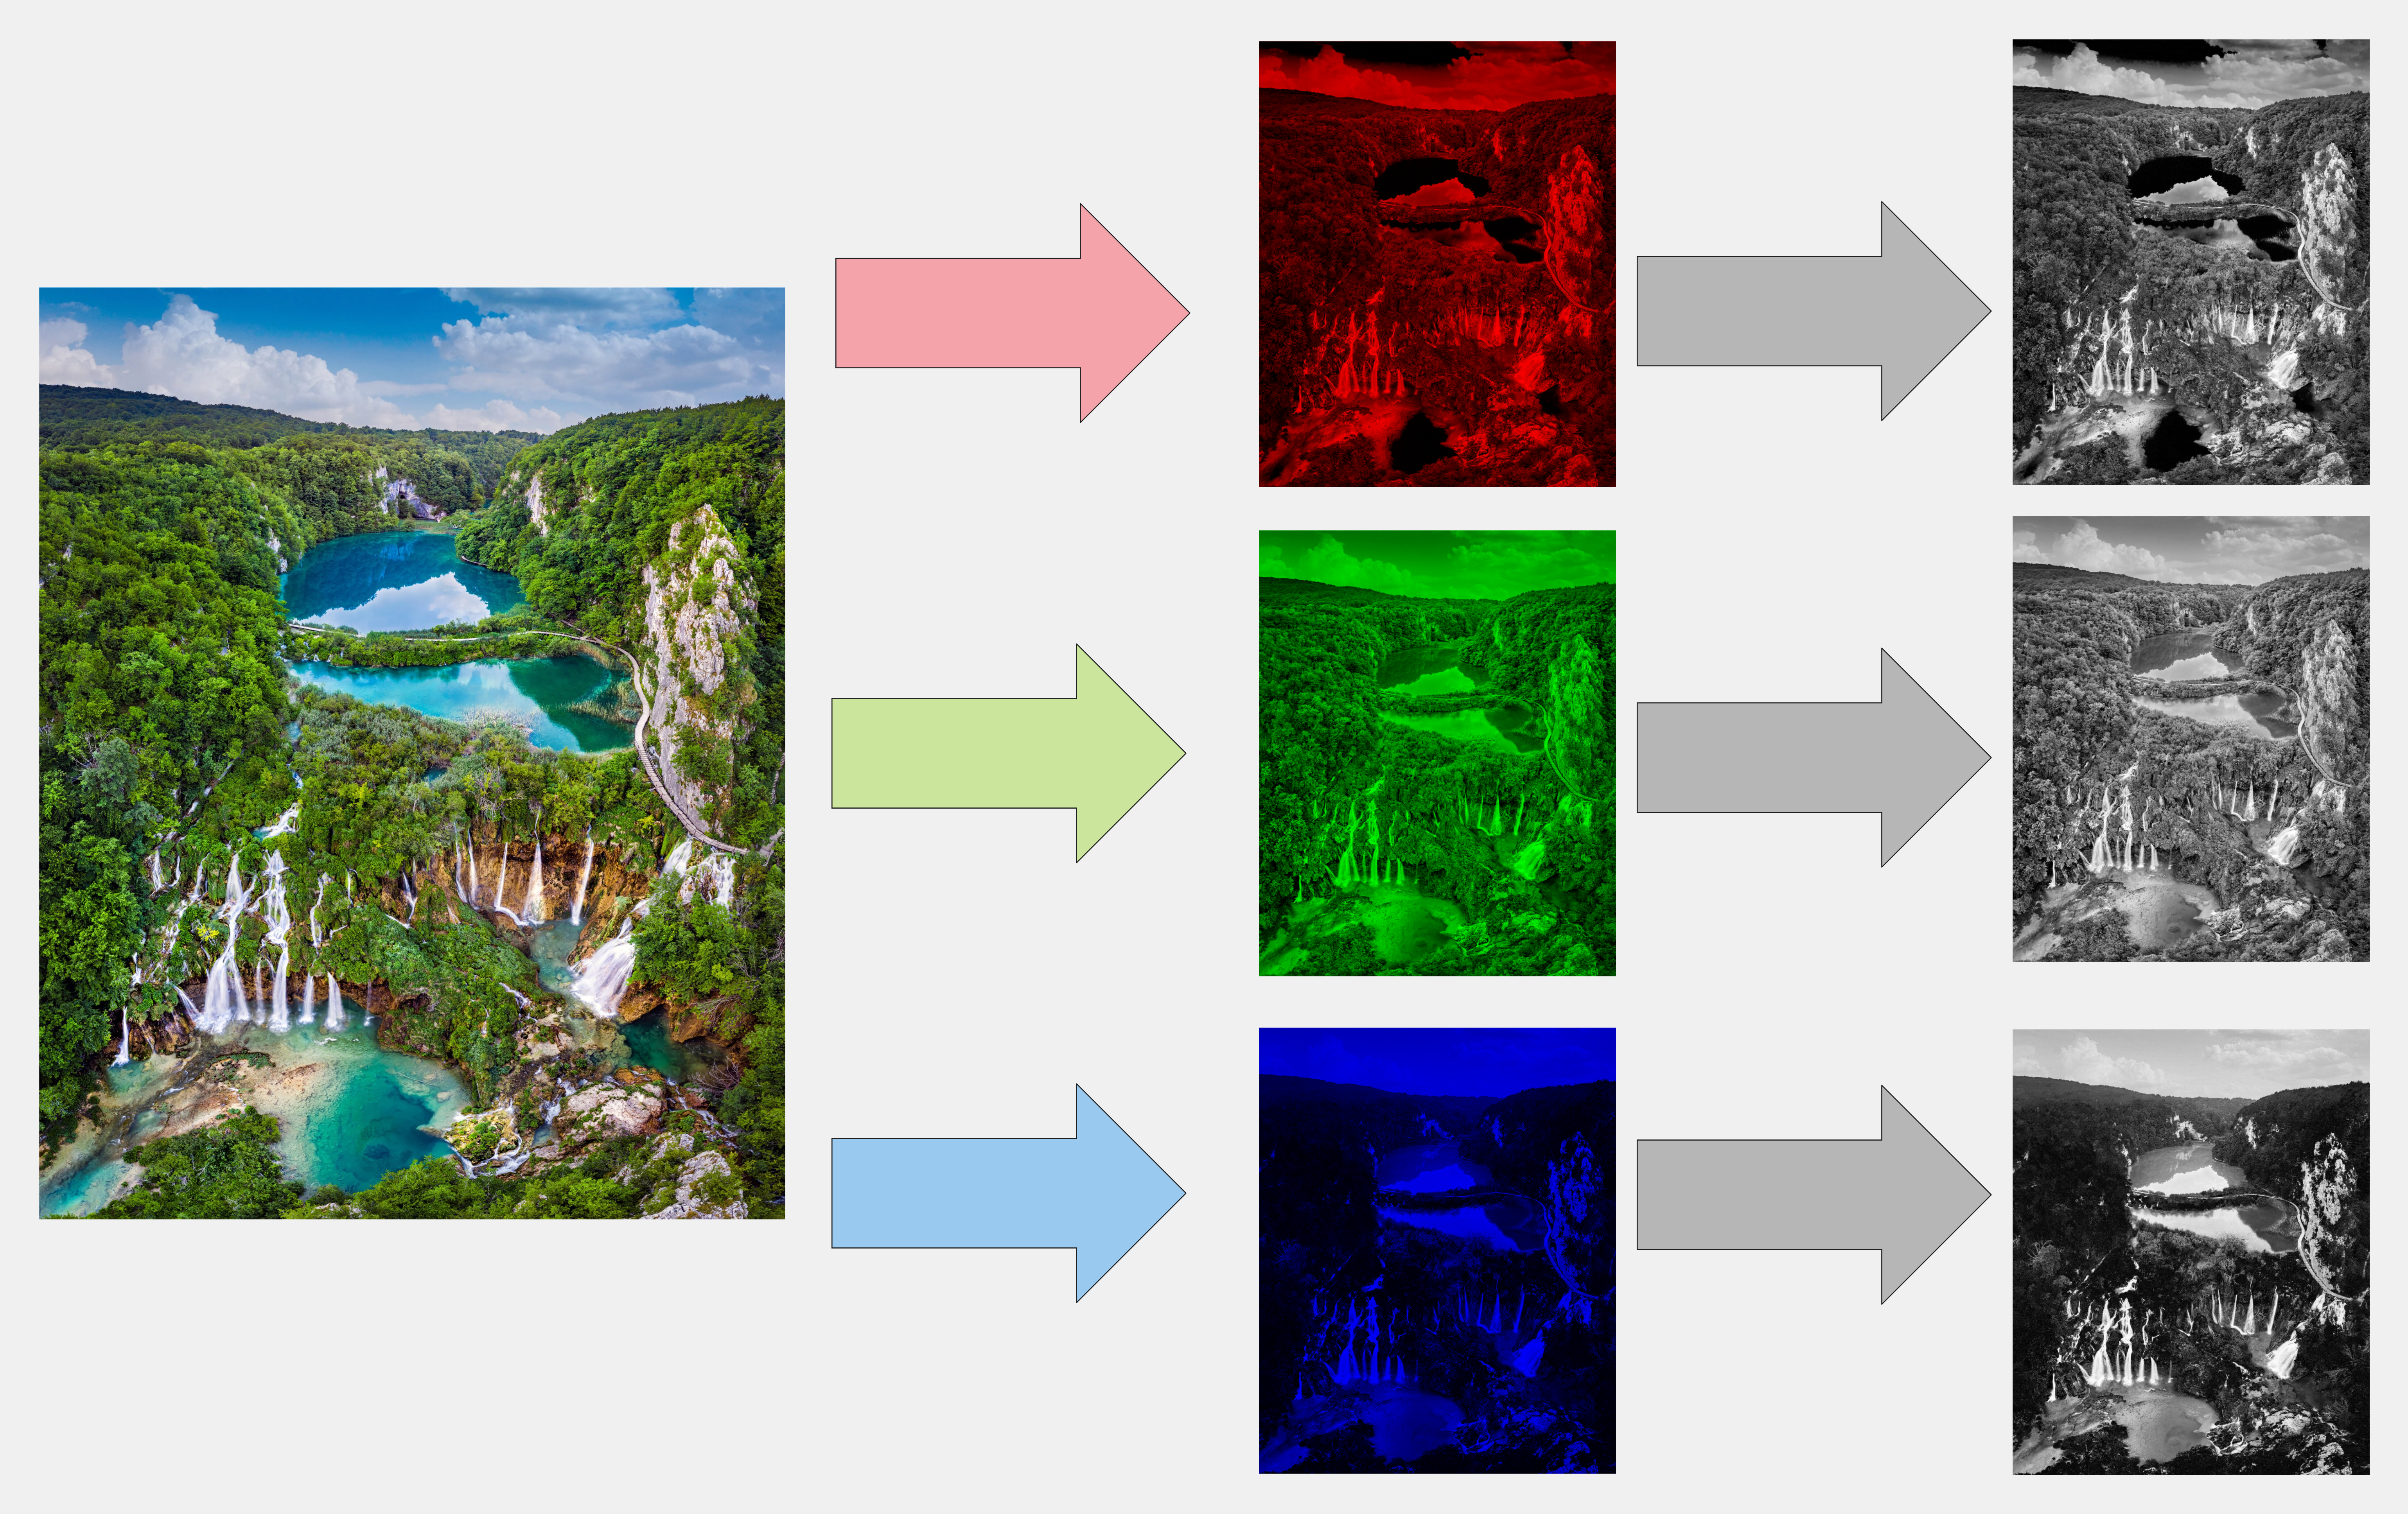
\includegraphics[width=1.0\linewidth]{slike/Color_chanell_separation.png}
    \caption{Prikaz slike u boji i pripadajućih kanala boja u rgb modelu (vlastita izrada)}
    \label{fig:channels}
\end{figure}

Kao što je prikazano na slici, kanali boja prikazani su kao slike čiji pikseli poprimaju boje samo crnu, bijelu i nijanse sive boje, takozvane sive slike. Također kanali se ponekad znaju vizualizirati pomoću primarne boje kanala kojeg reprezentiraju, ali sami podaci koje digitalna slika sadrži su uvijek jednaki, jedino način njihove vizualuizacije varira. 

\subsection{Sive slike}

Sive slike (\textit{eng. grayscale}) su poseban tip digitalnih slika koji ima samo jedan kanal boja. U tom kanalu vrijednosti piksela reprezentira svijetlinu piksela. Vizualizacija takvih slika poprima boje od bijele do crne uključujući nijanse sive. Na primjer za sliku sa dubinom boja od 8 bitova, nula bi predstavljala crnu boju, 255 bijelu, a vrijednosti između nijanse sive \cite{GrayscaleSlika}.

Sive slike su jedan od važnijih koncepata obrade slike i računalnog vida. One su zapravo baza mnogih algoritama za procesiranje slika. Često se korsite kao prvi korak obrade. Izrazito su korisne za detekciju rubova, segmentaciju slike, prepoznavanje uzorak i slično \cite{Grayscale2}. Kroz rad će se detaljnije prikazati njihova važnost i uloga u kontekstu detektiranja označenih odgovora na pismenim ispitima. 

\begin{figure}[H]
    \centering
    \includegraphics[width=0.7\linewidth]{slike/Grayscale.jpeg}
    \caption{Prikaz sive slike (vlastita izrada)}
\end{figure}

Na priloženoj sivoj slici se također može vidjeti da je različita od sivih slika kanala prikazanih na \hyperref[fig:channels]{slici 1}. To je zato što se kod pretvorbe slike u boji u sivu sliku kortsite vrijednosti sva 3 kanala prema formuli:

{\large
\[
    I_{\text{gray}}(x, y) = 0.299 \cdot R(x, y) + 0.587 \cdot G(x, y) + 0.114 \cdot B(x, y)\text{\cite{Grayscale2}}
\]
}


\subsection{Binarne slike}

Osim slika u boji i sivih slika također postoje i binarne slike. Binarne slike su tip slika gdje piksel može imati samo dvije moguću vrijednosti 0 i 1 od kud im dolazi i naziv. Binarne slike sadrže puno manje informacija od ostalih tipova slika, ali isto tako smanjuju kompleksnost same slike i omogućuju fokusiranje na važne značajke slike. Baš zbog toga se jako često koriste kod obrada slika koristeći računalni vid \cite{BinarySlika}.

\begin{figure}[H]
    \centering
    \includegraphics[width=0.75\linewidth]{slike/Binary.jpeg}
    \caption{Prikaz binarne slike (vlastita izrada)}
\end{figure}


Sam proces izrade binarne slike je dosta jednostavan. Za početak potrebno je imati sivu sliku. Zatim se definira granica (\textit{eng. treshold}) u obliku postotka. Ta granica se zatim koristi za određivanje vrijesnoti piksela, ako je vriejdnost iznad granice onda se vrijednost postavlja na jedan, a inaće na nulu. Priložena formula prikazuje osnovni tip kreiranja binarne slike (\textit{eng. tresholding}).

{\large
    \[
I_{\text{gray}}(x, y) = 0.299 \cdot R(x, y) + 0.587 \cdot G(x, y) + 0.114 \cdot B(x, y)
\]

\[
I_{\text{binary}}(x, y) =
\begin{cases}
1, & \text{if } I_{\text{gray}}(x, y) \geq T \\
0, & \text{if } I_{\text{gray}}(x, y) < T
\end{cases}
\]}


\subsection{Važnost različitih tipova digitalnih slika}

Do sada smo prošli kroz 3 najvažnija tipa digitalnih slika za ovaj rad. Kroz ovu cijelinu prikazat će se važnost pojedinog tipa slike naspram ostalih.

Zapravo najveća razlika između ovih tipova je broj kanala boje. Slike u boji imaju 3 kanala za razliku od sivih i binarnih slika koje imaju po jedan kanal. To zapravo znači da slike u boji sadrže značajno više informacija. 

No ponekad nam te informacije nisu potrebne ovisno o problemu koji pokušavamo rješiti. Na primjer ako pokušavamo detektirati boju svjetla na semaforu onda su nam informacije o bojama izrazito važne. No ako pokušavamo pročitati tekst sa prometnog znaka onda nam informacija o boji znaka i teksta ne doprinosi rješavanju problema. Zapravo nam otežava rješavanje problema pošto moramo raditi sa nepotrebnim informacijama.

\begin{figure}[H]
    \centering
    \includegraphics[width=1.0\linewidth]{slike/Luminace vs chrominance.png}
    \caption{Usporedba svijetloste komponente i komponenta boja(vlastita izrada)}
\end{figure}

Na priloženoj slici prikazana je ista slika na raličite načine:
\begin{itemize}
    \item Slika u RGB formatu
    \item Slika u YCbCr formatu
    \begin{itemize}
        \item Svijetlosne infromacije u Y kanalu
        \item Inforamcije o bojama u Cb i Cr kanalima
    \end{itemize}
  \end{itemize}

Na ovom primjeru je prikazana činejnica da svijetlosni kanali sadrže puno više informacija o strukturnim elementima na slici. baš zbog toga se u raznim algoritmima za detektiranje značajki, filtriranje, segmentiranje i sl. korsite baš sive slike \cite{LumVsChrom}. 

Sive slike se korsite kada boja nije važan faktor u obradi slike. U tom slučaju je boja jednako korisna kao buka na slici pa je zbog toga uklonimo. Time se veličina slike smanje i time ubrza daljni proces obrade slike \cite{LumVsChrom}.

Ako je potreban još agresivniji pristup otklanjanju nepotrebnih podataka onda binarne slike mogu postati korisne. One dodatno odstranjuju nepotrebe podatke tako da povećavaju razliku u kontrastu \cite{LumVsChrom}.

Važno je napomenuti da svaki tip slika ima svoju upotrebu ovisno o problemu koji se rješava. U ovom radu će veliku važnost imati sive i binarne slike pošto se radi o procesu detektiranja strukture fotografije i izvlačenja relevantnih informacija iz nje.


\section{Digitalna obrada slike}

Digitalna obrada slike podrazumijeva obradu digitalne fotografije koristeći računalne algoritme s ciljem unaprijeđivanja slike, izvlačenja korisnih informacija i sl.

Sam proces digitralne obrade slike može se podijeliti u 3 faze:
\begin{itemize}
\item Unos slike
\item Analiza i manipulacija slike
\item Generiranje resultata obrade slike
\end{itemize}



\subsection{Priprema slike}

\subsection{Pretvaranje u sivu sliku}

\subsection{Smanjenje buke}

\subsection{Pretvaranje u binarnu sliku}

\subsection{Detektiranje kontura}

\subsection{Detektiranje linija}

\subsection{Izvlačenje informacija iz slike}

\chapter{Zaključak}

Ovdje treba sažeto rezimirati najvažnije rezultate razrade teme rada. Potrebno je sažeto opisati što je predmet rada, koje su metode, tehnike, programski alati ili aplikacije korištene u razradi rada te koje su pretpostavke dokazane, a koje opovrgnute. Sadržajno, ono što se u uvodu rada najavljuje i kasnije je obuhvaćeno u samom radu, moralo bi biti opisano u zaključnom dijelu kroz rezultate rada. 


\printbibliography[title=Popis literature]
\addcontentsline{toc}{chapter}{Popis literature}

\listoffigures
\addcontentsline{toc}{chapter}{Popis slika}
 
\listoftables
\addcontentsline{toc}{chapter}{Popis popis tablica}

\appendix
\renewcommand{\thechapter}{\arabic{chapter}}


\end{document}
